\documentclass[letterpaper,10pt,titlepage]{IEEEtran}
\usepackage{lipsum}
\usepackage{graphicx}
\usepackage{amssymb}
\usepackage{amsmath}
\usepackage{amsthm}

\usepackage{alltt}
\usepackage{float}
\usepackage{color}
\usepackage{url}
\usepackage{listings}
\lstset{ 
   language=C++,                % choose the language of the code
   basicstyle=\small,        % the size of the fonts that are used for the code
   keywordstyle=\color{blue},
   stringstyle=\color{red},
   commentstyle=\color{green},
   numbers=left,                   % where to put the line-numbers
   numberstyle=\footnotesize,      % the size of the fonts that are used for the line-numbers
   stepnumber=1,                   % the step between two line-numbers. If it is 1 each line will be numbered
   numbersep=5pt,                  % how far the line-numbers are from the code
   backgroundcolor=\color{white},  % choose the background color. You must add \usepackage{color}
   showspaces=false,               % show spaces adding particular underscores
   showstringspaces=false,         % underline spaces within strings
   showtabs=false,                 % show tabs within strings adding particular underscores
   frame=single,           % adds a frame around the code
   tabsize=2,          % sets default tabsize to 2 spaces
   captionpos=b,           % sets the caption-position to bottom
   breaklines=true,        % sets automatic line breaking
   breakatwhitespace=false,    % sets if automatic breaks should only happen at whitespace
   escapeinside={\%*}{*)}          % if you want to add a comment within your code
   }
   \usepackage{balance}
   \usepackage[TABBOTCAP, tight]{subfigure}
   \usepackage{enumitem}
   \usepackage{pstricks, pst-node}

   \usepackage{geometry}
   \usepackage{longtable,hyperref}
   \geometry{textheight=8.5in, textwidth=6in, margin=0.75in}

   %\graphicspath{ /nfs/stak/students/p/palmiteh/CS461/Winter_Midterm/ }
 
   \renewcommand*\rmdefault{cmr}

   \newcommand{\cred}[1]{{\color{red}#1}}
   \newcommand{\cblue}[1]{{\color{blue}#1}}
   \newcommand{\itab}[1]{\hspace{4em}\rlap{#1}}


   \title{Spring Term Progress Report}
   \author{Hailey Palmiter, Scott Griffy, and Ryan Kitchen}
   \date{\today}

   %% The following metadata will show up in the PDF properties
   \hypersetup{
      colorlinks = true,
      urlcolor = black,
      pdfauthor = {Palmiter, Griffy, Kitchen},
      pdftitle = {Spring Term Progress Report},
      pdfsubject = {CS462},
      pdfpagemode = UseNone
   }
   \begin{document}
   \begin{titlepage}
      \centering
      \vfill
      {\bfseries\Large
         Spring Term Progress Report \\
         CS 462 - Senior Capstone\\
         \vskip2cm
         March 16th, 2016\\
         \vskip2cm
         The HawkEyed Crew - Group 4\\ 
         \vskip1cm
         Hailey Palmiter\\
         \vskip1cm
         Scott Griffy\\
         \vskip1cm
         Ryan Kitchen\\
    
      }
      \vfill
      \vskip2cm
      \begin{abstract}
      This document is a release progress report that covers a brief introduction of our senior project, our current progress, problems that have impeded our progress, and the results that have been gathered. It also describes what is left to do to increase our projects performance and/or create more concrete testing of our software system before it is presented at the Engineering Expo. It also describes our stretch goals may complete before then as well and some detail about our planning of our demo for expo. This report includes a few interesting pieces of code and a description of what this code does to improve or enhance our system. It is constructed using the IEEEtran style guidelines.
      \end{abstract}
      \vfill
   \end{titlepage}
   
   \onecolumn
   \tableofcontents
   \newpage
   \bigskip
   \section{Introduction}
   Rockwell Collins, our project sponsor, designs video vision systems for pilots to use during flight. Pilots often use these enhanced image systems to help them see better in rough weather conditions, and to generally assist during different flight operations, such as landing. An example of this functionality could be overlaying a pilot's view with graphics to help the pilot locate a landing strip in a storm, or automatically turning a night-vision camera off when it is not needed to save power. The hardware used for this system must limit the power consumption it pulls from the aircraft, and also must be lightweight in order to have the least affect on the airplane. Even an extra five pounds added to the plane during a year can add up to thousands of dollars in fuel costs. In order to provide pilots with this specific low power, low weight, and enhanced image processing, Rockwell Collins develops software on Field Programmable Gate Arrays (FPGAs). This piece of hardware makes the code very complex and very costly to develop. New vision enhancements can take weeks or months to develop on the FPGAs. The FPGAs are currently Rockwell Collins only option that meets the requirements needed to create practical systems that pilots can use effectively.\\
\par
   Our goal is to provide a proof of concept for an alternative to Rockwell Collins' FPGAs. It must meet the performance metrics, provide faster implementation time, and reduce the cost of production. Specifically, we are designing a proof of concept using single board computers (SBCs). Single board computers differ from FPGAs because they have a standardized execution environment, which allows simplified code to be executed on it, reducing the development time. Single board computers also use low cost hardware and don't consume much power. If we can prove that the video quality produced by the SBCs is adequate for pilots to use, they will meet all the requirements needed to develop a practical vision system on. In the air, FPGAs often take feeds from multiple cameras and run a lot of processing algorithms on those images. In order to be effective, the SBCs should also be able to handle this operation. Our project aims to test and measure the capabilities of a single board computer by delivering a multiple-stream video display that has been processed to a high degree. We believe the best candidate for this is to use NVIDIA's single board computer, the Jetson TX1. Our goal is to fully test the Jetson TX1's ability to provide enhanced imaging. This proof of concept will result in measurements that will help Rockwell Collins determine the practicality of using single board computers for their vision systems.
   
\section{Hardware}
   This section includes a list of all the hardware we have been (very generously) lent and have been working with for the duration of this project. The following list and images should be able to supply a better understanding and familiarization of the project.\\
	\\Cameras (figure 1):  
    		\begin{itemize}
		\item GS3-U3-41C6NIR-C (PointGrey/GrassHopper)
		\item GS3-U3-41C6C-C
		\item GS3-U3-23S6C-C\\
		\end{itemize}
	Lenses (figure 1): 
		\begin{itemize}
		\item EVS-3000 (figure 6)
		\item 2 x LS-TP-08 (Standard) (figure 7)\\
		\end{itemize}
		
\begin{figure}[!ht]
  \caption{The 3 cameras provided by Rockwell Collins on a mount}
	  \centering
		    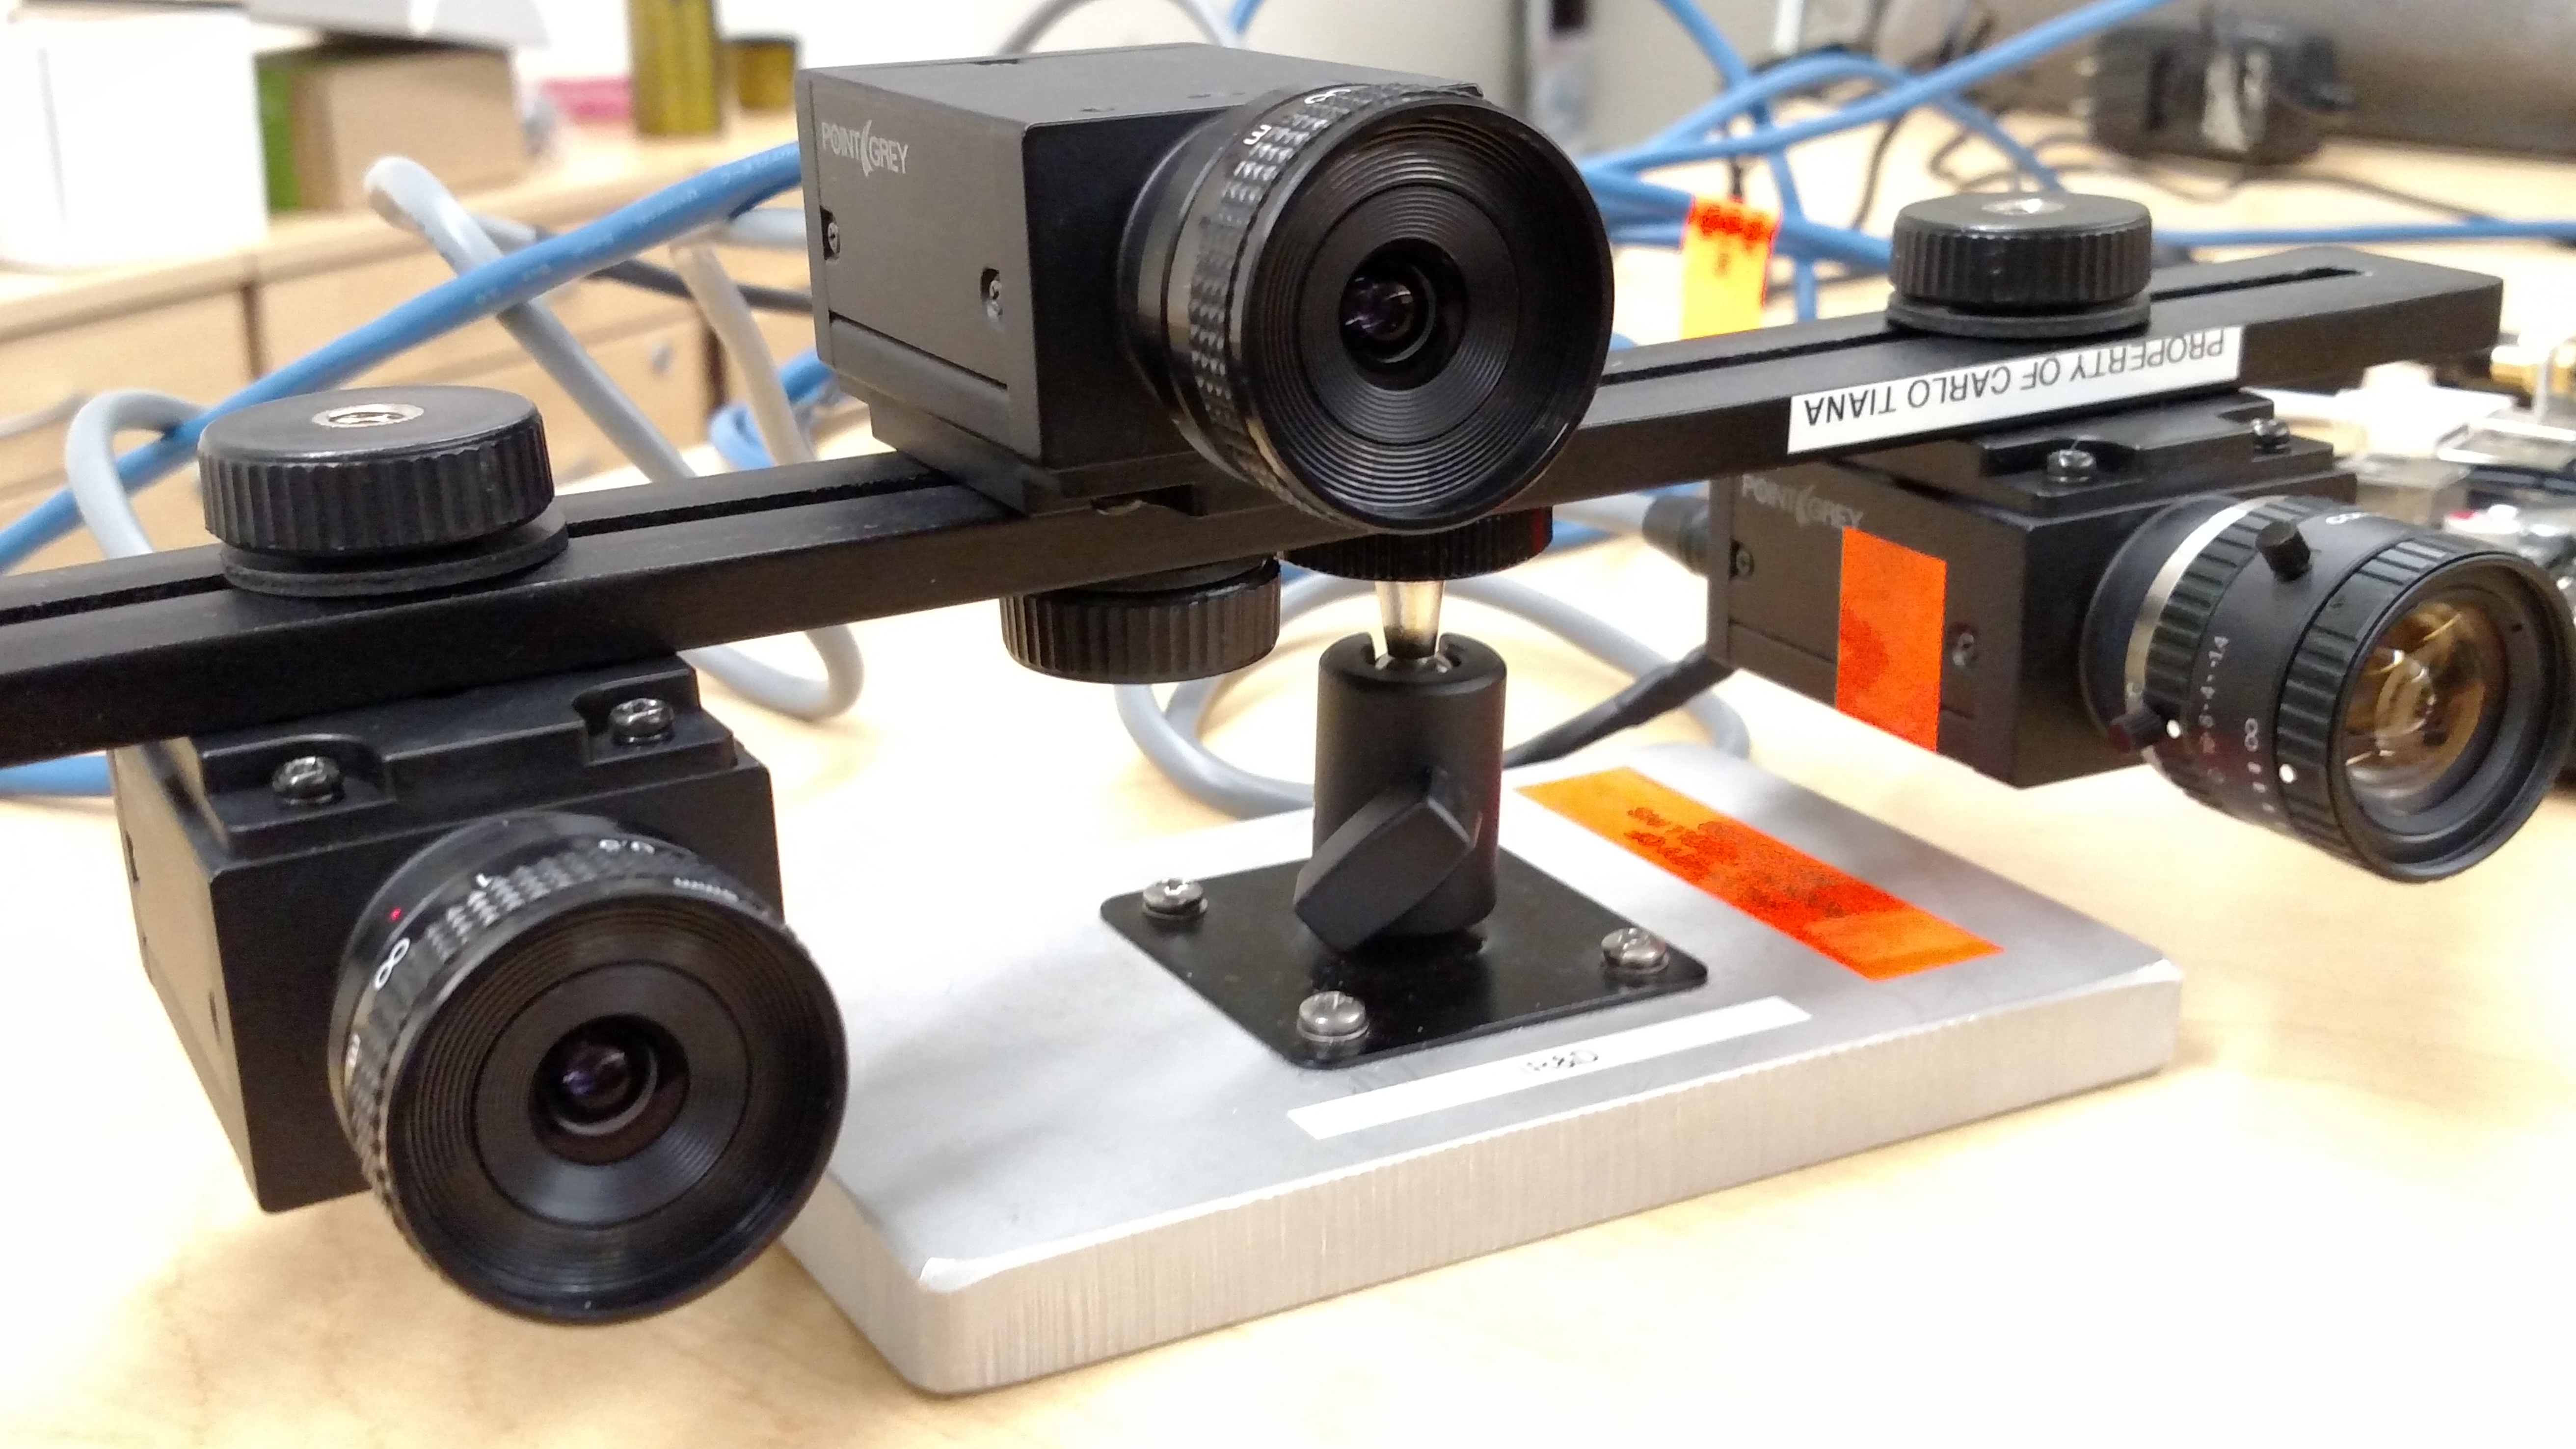
\includegraphics[width=0.6\textwidth,natwidth=610,natheight=642]{images/IMG_20160210_131527329.jpg}
				\end{figure}
				
	Single Board Computers: 
		\begin{itemize}
		\item Jetson TK1 (figure 2) 
		\item Jetson TX1 developer kit with on-board camera (figure 3 and 4)\\
		\end{itemize}
 
 \begin{figure}[!ht]
  \caption{The Jetson TK1}
	  \centering
		    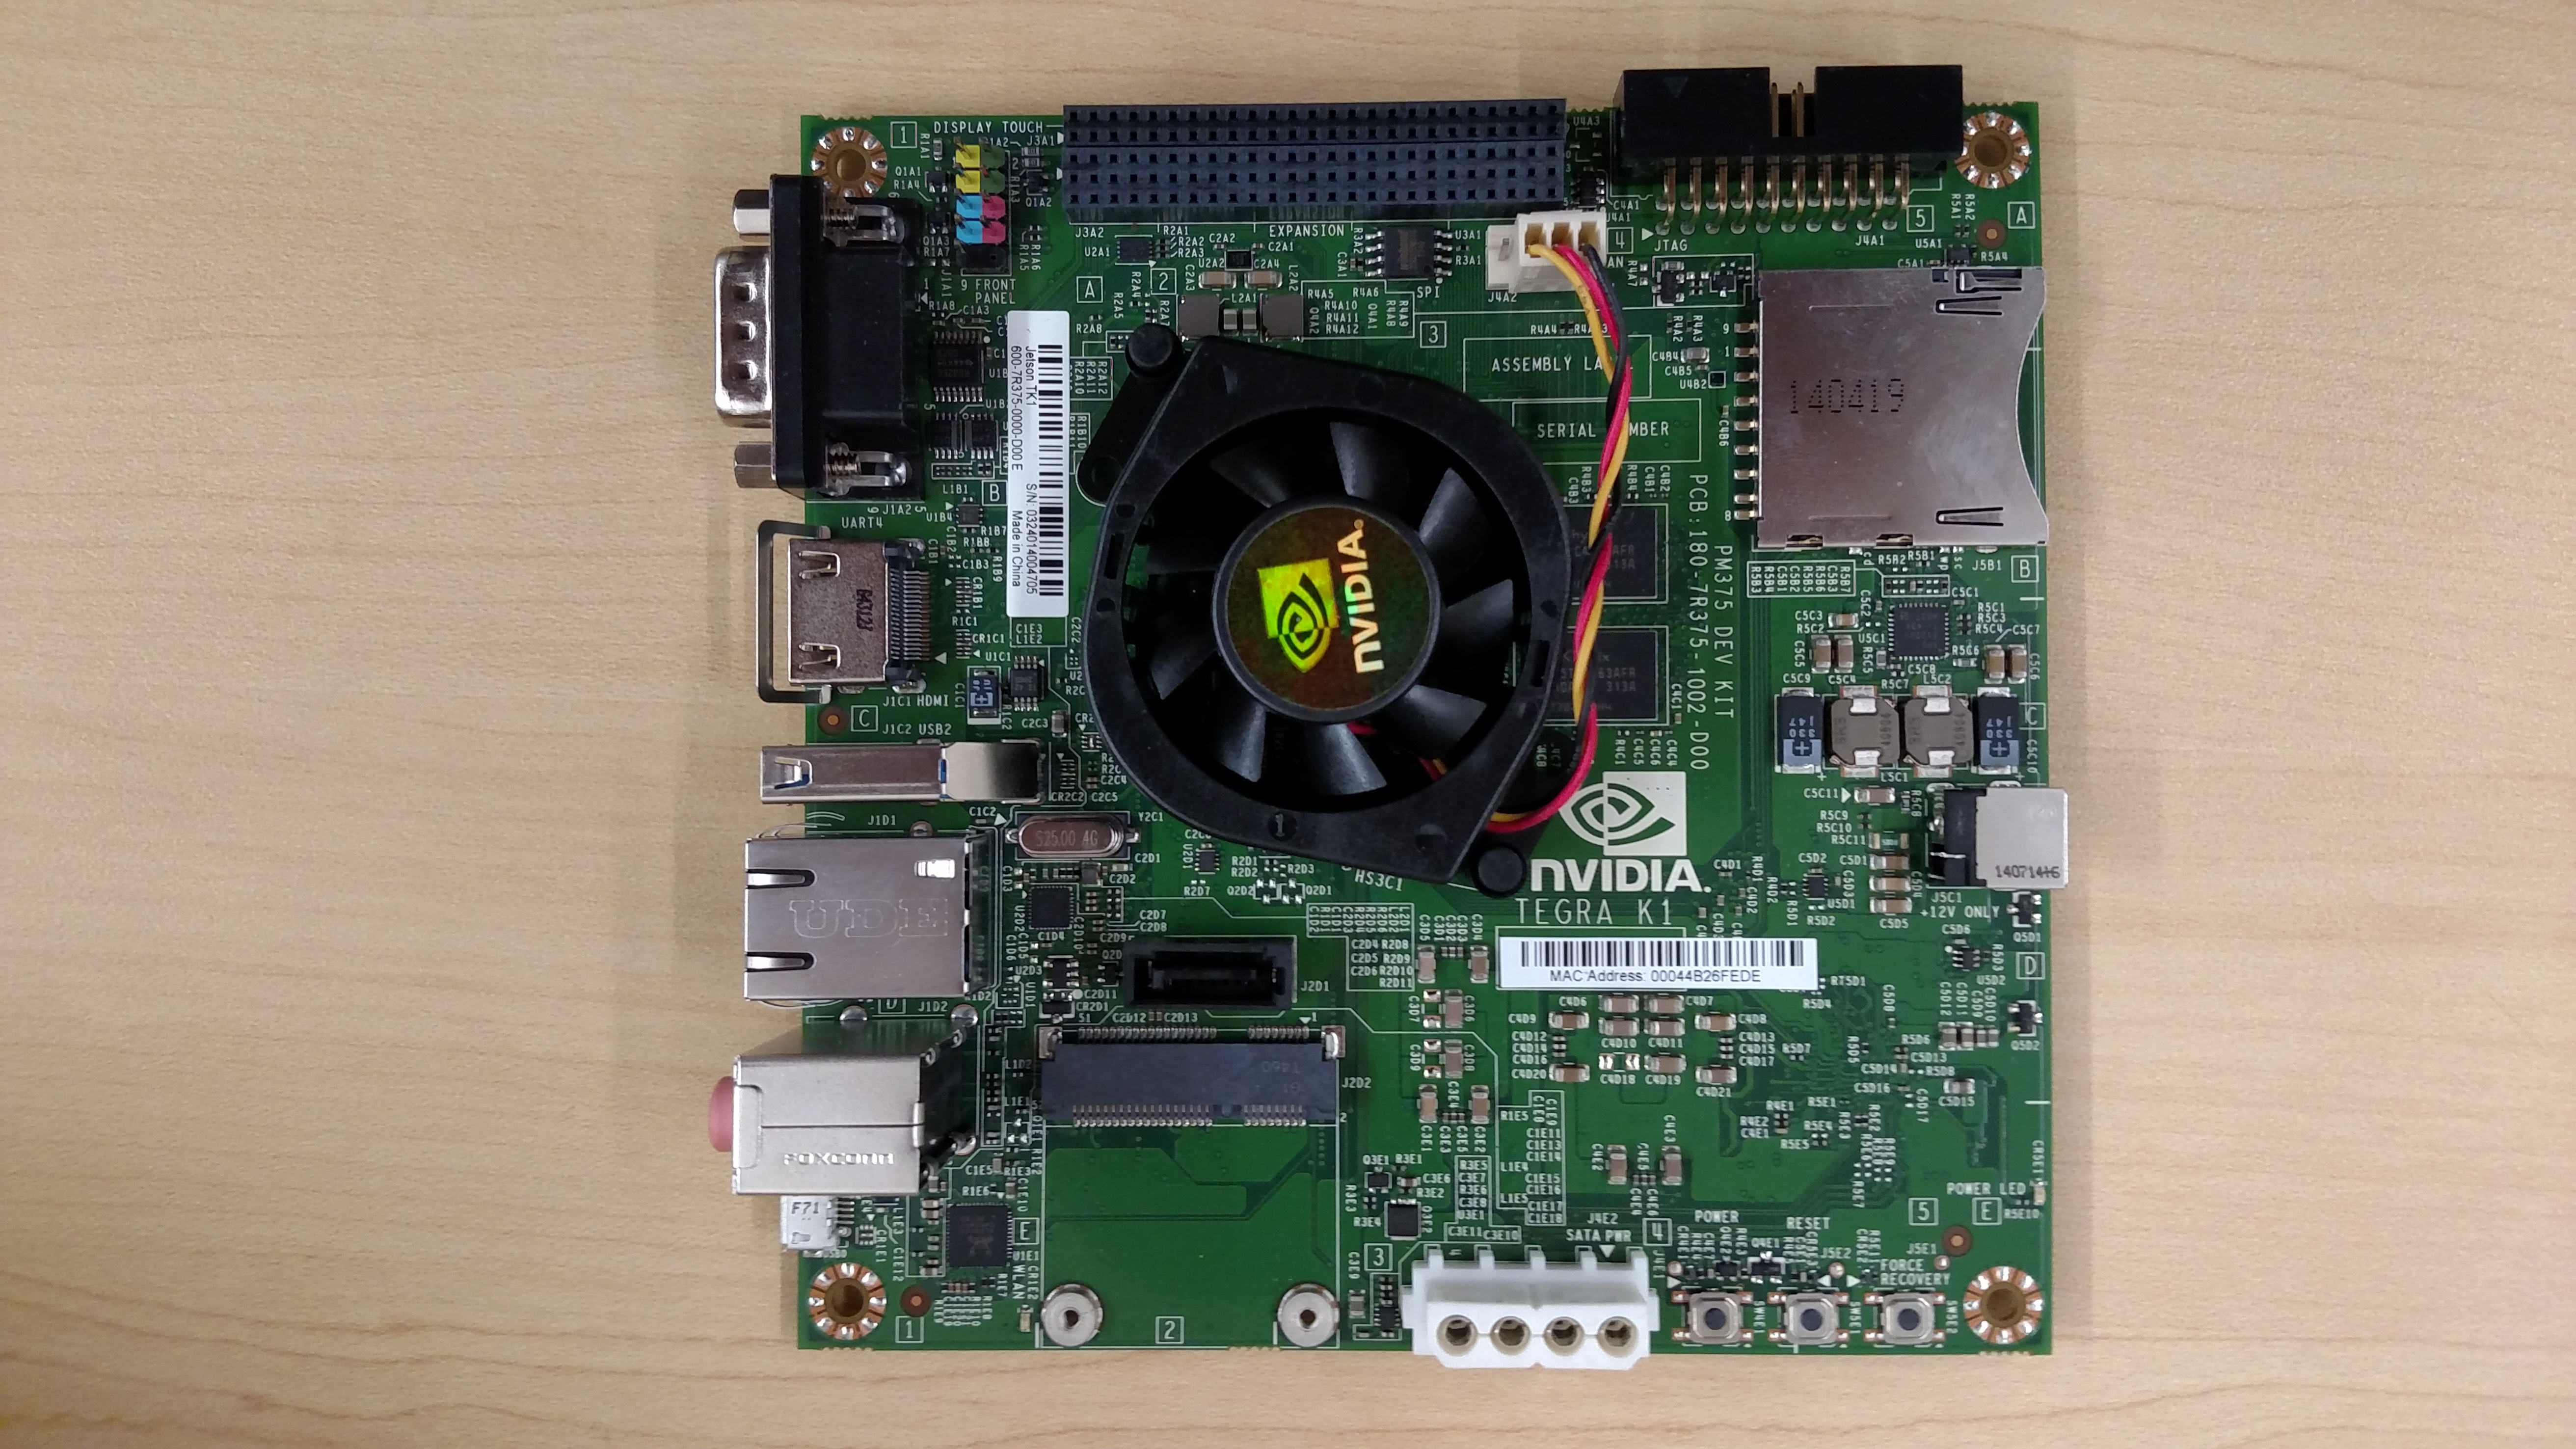
\includegraphics[width=0.6\textwidth,natwidth=610,natheight=642]{images/rot-9.jpg}
				\end{figure}
\begin{figure}[!ht]
  \caption{The Jetson TX1}
	  \centering
		    \includegraphics[width=0.6\textwidth,natwidth=610,natheight=642]{images/rot-8.jpg}
				\end{figure}
\begin{figure}[!ht]
  \caption{The on-board camera for the TX1}
	  \centering
		    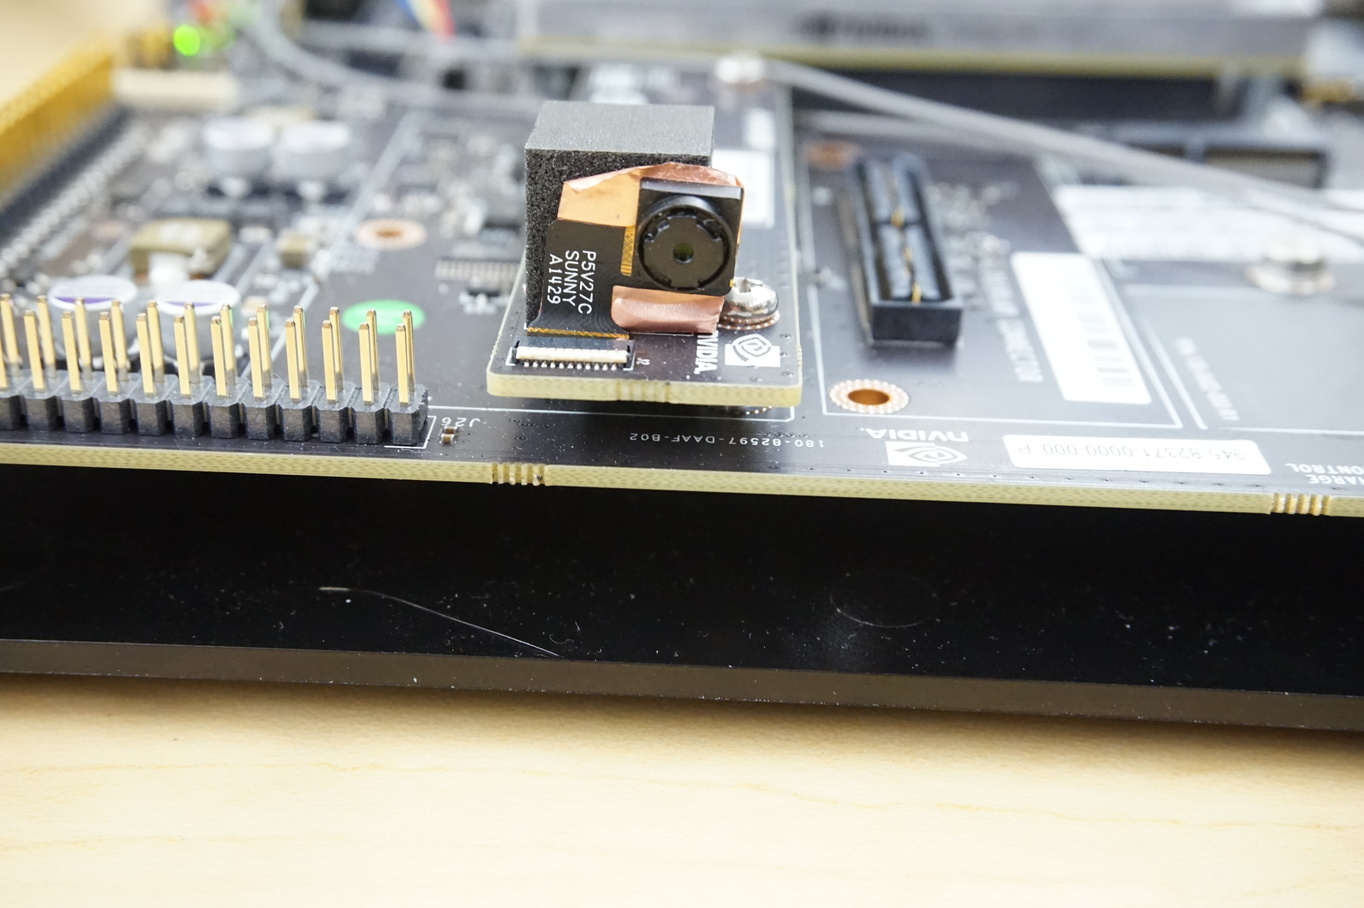
\includegraphics[width=0.6\textwidth,natwidth=610,natheight=642]{images/onboardCamera.JPG}
				\end{figure}
	Extras: 
		\begin{itemize}
		\item NIR Pass filter - blocks visible light while allowing NIR light through
		\item 2-port USB 3.0 supersede PCIe Card (figure 5)
		\item Camera mount
		\item 3 x USB 3.0 cables
		\item 1080p monitor (TV)\\
		\end{itemize}

\begin{figure}[!ht]
  \caption{2-port USB 3.0 supersede PCIe Card}
	  \centering
		    \includegraphics[width=0.6\textwidth,natwidth=610,natheight=642]{images/PCIe.jpg}
				\end{figure}


\section{Progress timeline}

   \subsection{Refined Requirements Document}
   Before real development began, we had reread our requirements document and noticed that some changes and additions needed to be made. The revision was needed in order to refine our project with the discovery of problems/improvements we had found. It was a needed process as we wanted to have full clarity on what needed to be accomplished with this project, and be able to display those requirements with our sponsor. The changes were reviewed with our sponsor and agreed upon before any final changes were made. The most current requirements document was uploaded to the SharePoint as Revised\_ReqDoc on January 15th, 2016.\\ 
\par
Only a few minor things were changed, but they had a big impact on how we define our deliverable according to their standard. Our client was very happy to see the revisions we had made and all final revisions were agreed upon. Theses changes included that we have two working cameras for our final system, and to use either the Jetson TK1 or the Jetson TX1 for development. Before the revision, the requirements document was specifying the use of only the Jetson TK1. After much research on our end we had decided that either Jetson's TK1 or TX1 would be adequate for development, and actually plan to rely more heavily on the Jetson TX1. This change allows us to have more flexibility between the two Jetson SBC's, which provides protection if we cannot get one to work properly or to the meet the requirements needed. 
   
   \subsection{Jetson TK1}
   We first began development on the Jetson TK1, as it was what we had on hand while we were waiting for the TX1 to arrive. We had installed graphics drivers on the TK1 as well as a driver for the original PointGrey camera we were loaned by Rockwell Collins. We had much difficulty working with the USB 3.0 port, due to the fact that the kernel support for it was disabled. We found that the Jetson TK1's operating system had to be recompiled in order to grab full 2048x2048 pixel images from the camera. Without the recompiled kernel we were able to grab images at a lower resolution using the FlyCapture API, and could only utilize the PointGrey camera as a USB 2.0 device, not USB 3.0. Even after the recompile of the kernel we still had connection issues and display latency with the video. We quickly began to realize that development on the TK1 may not even be worth the struggle, and have moved our development process to the TX1.\\ 
\par
It would be possible to continue development on the TK1, but it does not seem to be the best option to obtain the greatest results moving forward with development. If time permits we will test our software system on the TK1 to measure its capabilities in comparison with the Jetson TX1.
   
   \subsection{Jetson TX1}
   After discovering a manufacturer error on the original TX1, we continued development on the TK1 until the new, fully functional, TX1 had arrived. This was the point when development had completely shifted from the TK1 to the TX1.\\
   
   \subsubsection{OpenCV Video Output}
   Our first step in exploring the Jetson TX1's capabilities, was to get a working video output from the on-board camera. We were able to display this image at 1080p with the option of either 30 or 60 frames per second. This video stream used embedded GStreamer code to transform the image buffer, generated from the camera, into a Video4Linux compatible format. The image was then read with a standard linux application and displayed to the monitor. After we were able to get the video output from the on-board camera, our next focus was on getting two cameras' video streams displayed to the monitor. This would allow us to be able to begin developing our software to handle processing of multiple video streams into one output. At the time we only currently had one USB 3.0 camera, but found that trying to combine the on-board camera with the PointGrey camera was going to be very difficult and would most likely have undesirable results. We decided that using two USB 3.0 cameras would be the best way to proceed in order to accomplish our needed performance metrics. While we were waiting for a second USB 3.0 camera from Rockwell Collins, we were able to display the one PointGrey camera stream onto our monitor. Figure 6 is an unprocessed output stream using the EVS-3000 lens and figure 7 is using the standard LS-TP-08 lens. We were even able to implement two basic edge detection functions using several of OpenCV's built-in filters and apply it to our output video. Figure 8 below demonstrates one of our edge detection filters applied to our output video stream.\\
   
   \begin{figure}[!ht]
  \caption{Video output from the TX1 using a PointGrey camera with an EVS-3000 lens attached}
	  \centering
		    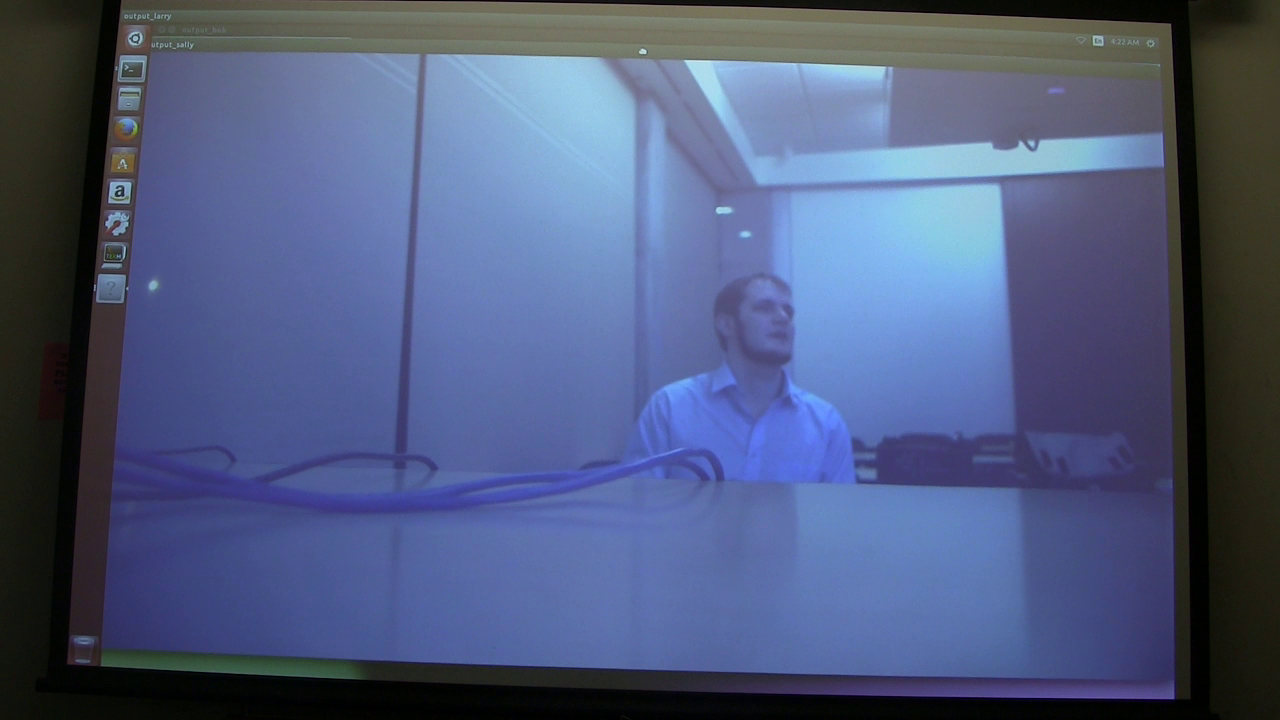
\includegraphics[width=0.6\textwidth]{images/vlcsnap-2016-02-11-17h42m53s150.png}
				\end{figure}
\begin{figure}[!ht]
  \caption{Video output from the TX1 using a PointGrey camera with a LS-TP-08 lens attached}
	  \centering
		    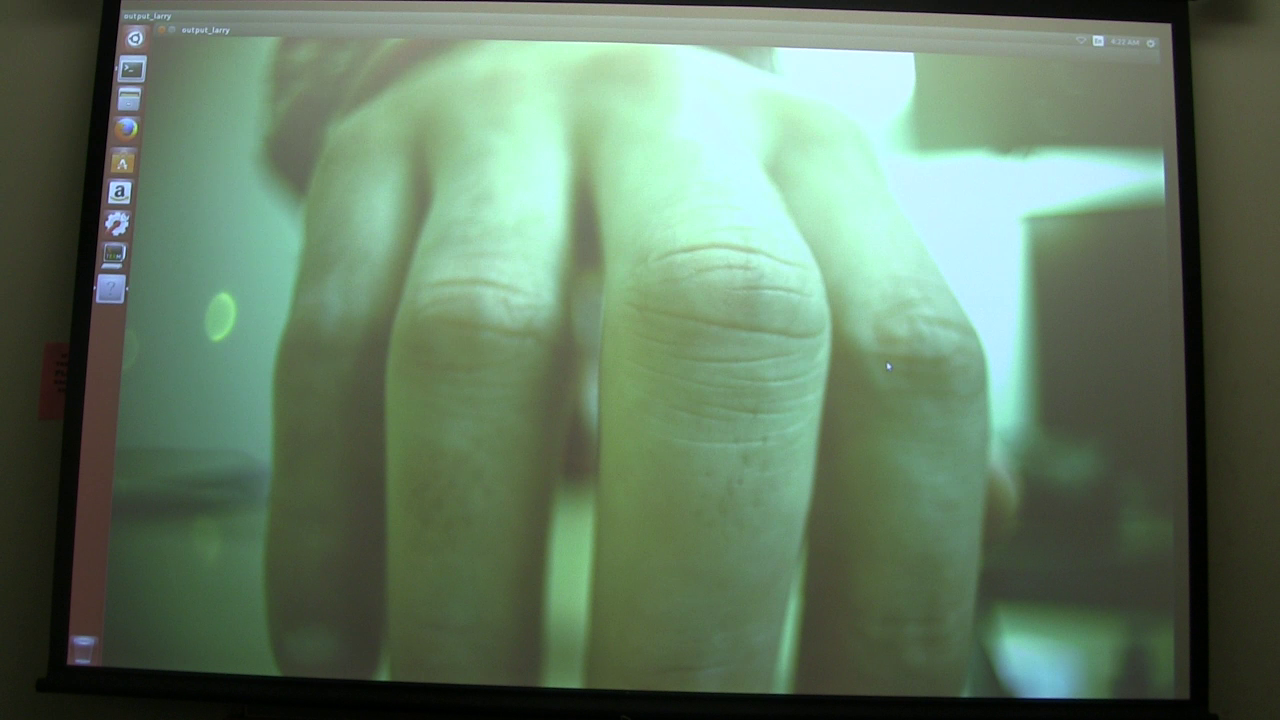
\includegraphics[width=0.6\textwidth]{images/vlcsnap-2016-02-11-17h42m30s486.png}
				\end{figure}
\begin{figure}[!ht]
  \caption{Video output from the TX1 using a built-in OpenCV line detection filter}
	  \centering
		    \includegraphics[width=0.6\textwidth]{images/line_detection.png}
				\end{figure}
   
   \subsubsection{OpenGL Video Output}
	We started using OpenCV because it was an easy framework to use. OpenCV could store the camera buffers, perform processing, and create a user interface that allowed us to see the video output stream. While this provided us with simplicity and easy development, the performance was well below out requirements. This was because OpenCV did not make use of the hardware on the Jetson. Part of this was because of OpenCV's poor implementation of copying the video buffer to the screen. In order to fully make use of the Jetson's hardware, we decided to switch to using an OpenGL framework, using GLUT, for creating the window and displaying the video. Our first implementation of an OpenGL system was still resulting in a slow image output. This was only because we were not exploiting the full capabilities that GLUT had to offer. GLUT has a zero copy function that allowed for us to not have to perform any memory copy operations. Once we had a better understanding of how to create and manipulate shared buffer space between the GPU and CPU, we were able to get much better output results. We then modified it to make better use of the hardware linking user buffers with the FlyCapture API to GPU textures. Our final product in this beta release ended up using an OpenGL framework to produce our highest performing result.\\

  \subsubsection{CUDA Library Functionality}
   After making use of the OpenGL framework to capture and display images we still needed a library to handle the processing of the images. We decided that NVIDIA's CUDA library would be adequate for the processing we needed to handle. We then installed the CUDA drivers and example code onto the Jetson TX1. CUDA includes a library and tool-chain that allows us to compile code that runs directly on the GPU called 'CUDA Kernels'. We can call these CUDA Kernels from our main thread in our software. This GPU compiled code can easily handle filters like line detection and much more. We are even planning to do a color space conversion using these CUDA Kernels. The CUDA package also came with some examples that were very useful in creating code spikes. The examples were very helpful and made our final code easier to write. We have rewritten and combined many of these examples to get the beta code working. Our results consisted in being able to overlay an outline detection image overtop of a separate camera's normal image.\\

   \subsubsection{Modular Software System}
   In order to create modularity and flexibility, we implemented a modular software architecture for our vision system. Our software reads a JSON configuration file to set-up the modules. Each module is comprised of a series of camera captures, filters, and sinks (displays). This module system allows for configuration without the need to recompile every time, which can be complex and time consuming. It also gives us the ability to implement different filter modules and quickly apply only the desired filters at a given time. We have plans to expand the system so that it could intelligently use different types of cameras only for specific reasons to conserve power consumption. An example could be that a long-range camera may only be activated when needed to find the runway from a given distance. It could then be turned on and processed when needed, but deactivated to increase the performance when it is not needed. We also want to implement a multiple camera overlay. An example of this system is having one camera capture the normal image while an infrared camera is detecting bright spots (i.e. runway lights). Once the camera filter has detected the bright lights, it then draws circles around each spot to make a clear indication of where a runway is. This image is then overlaid onto the normal image to give the pilots the best possible accuracy and location of the runway. The impact of the flexibility of this modular system is limitless for being able to assist in safe flight in almost all situations.\\
   
   \subsubsection{Development of the Modules}
Development of this system is an iterative process. We first explored the modular system by outputting a static image to demonstrate that the system was working. We then created a module to handle input from the PointGrey camera by implementing its given software. This allowed us to be able to interact with multiple PointGrey cameras. When we received the USB 3.0 PCIe card, we were able to implement up to three cameras at once over USB 3.0, all overlaying their video streams on top of each other to provide one output stream. Currently we have it set up so that one camera is providing 50\% of the display output and the other two are split by 25\% each. When only two cameras are running, the video output is provided with a split 50\% input from the cameras equally. The results of this output video stream is shown in figure 9 below. We have also added a line detection filter, which can run without dropping our frame rate any significant amount. The ability and ease of being able to switch between how many cameras are running and applying filters to each has proven the efficiency of our modular system. 

\begin{figure}[!ht]
  \caption{Video output from the TX1 overlaying three USB 3.0 video streams}
	  \centering
		    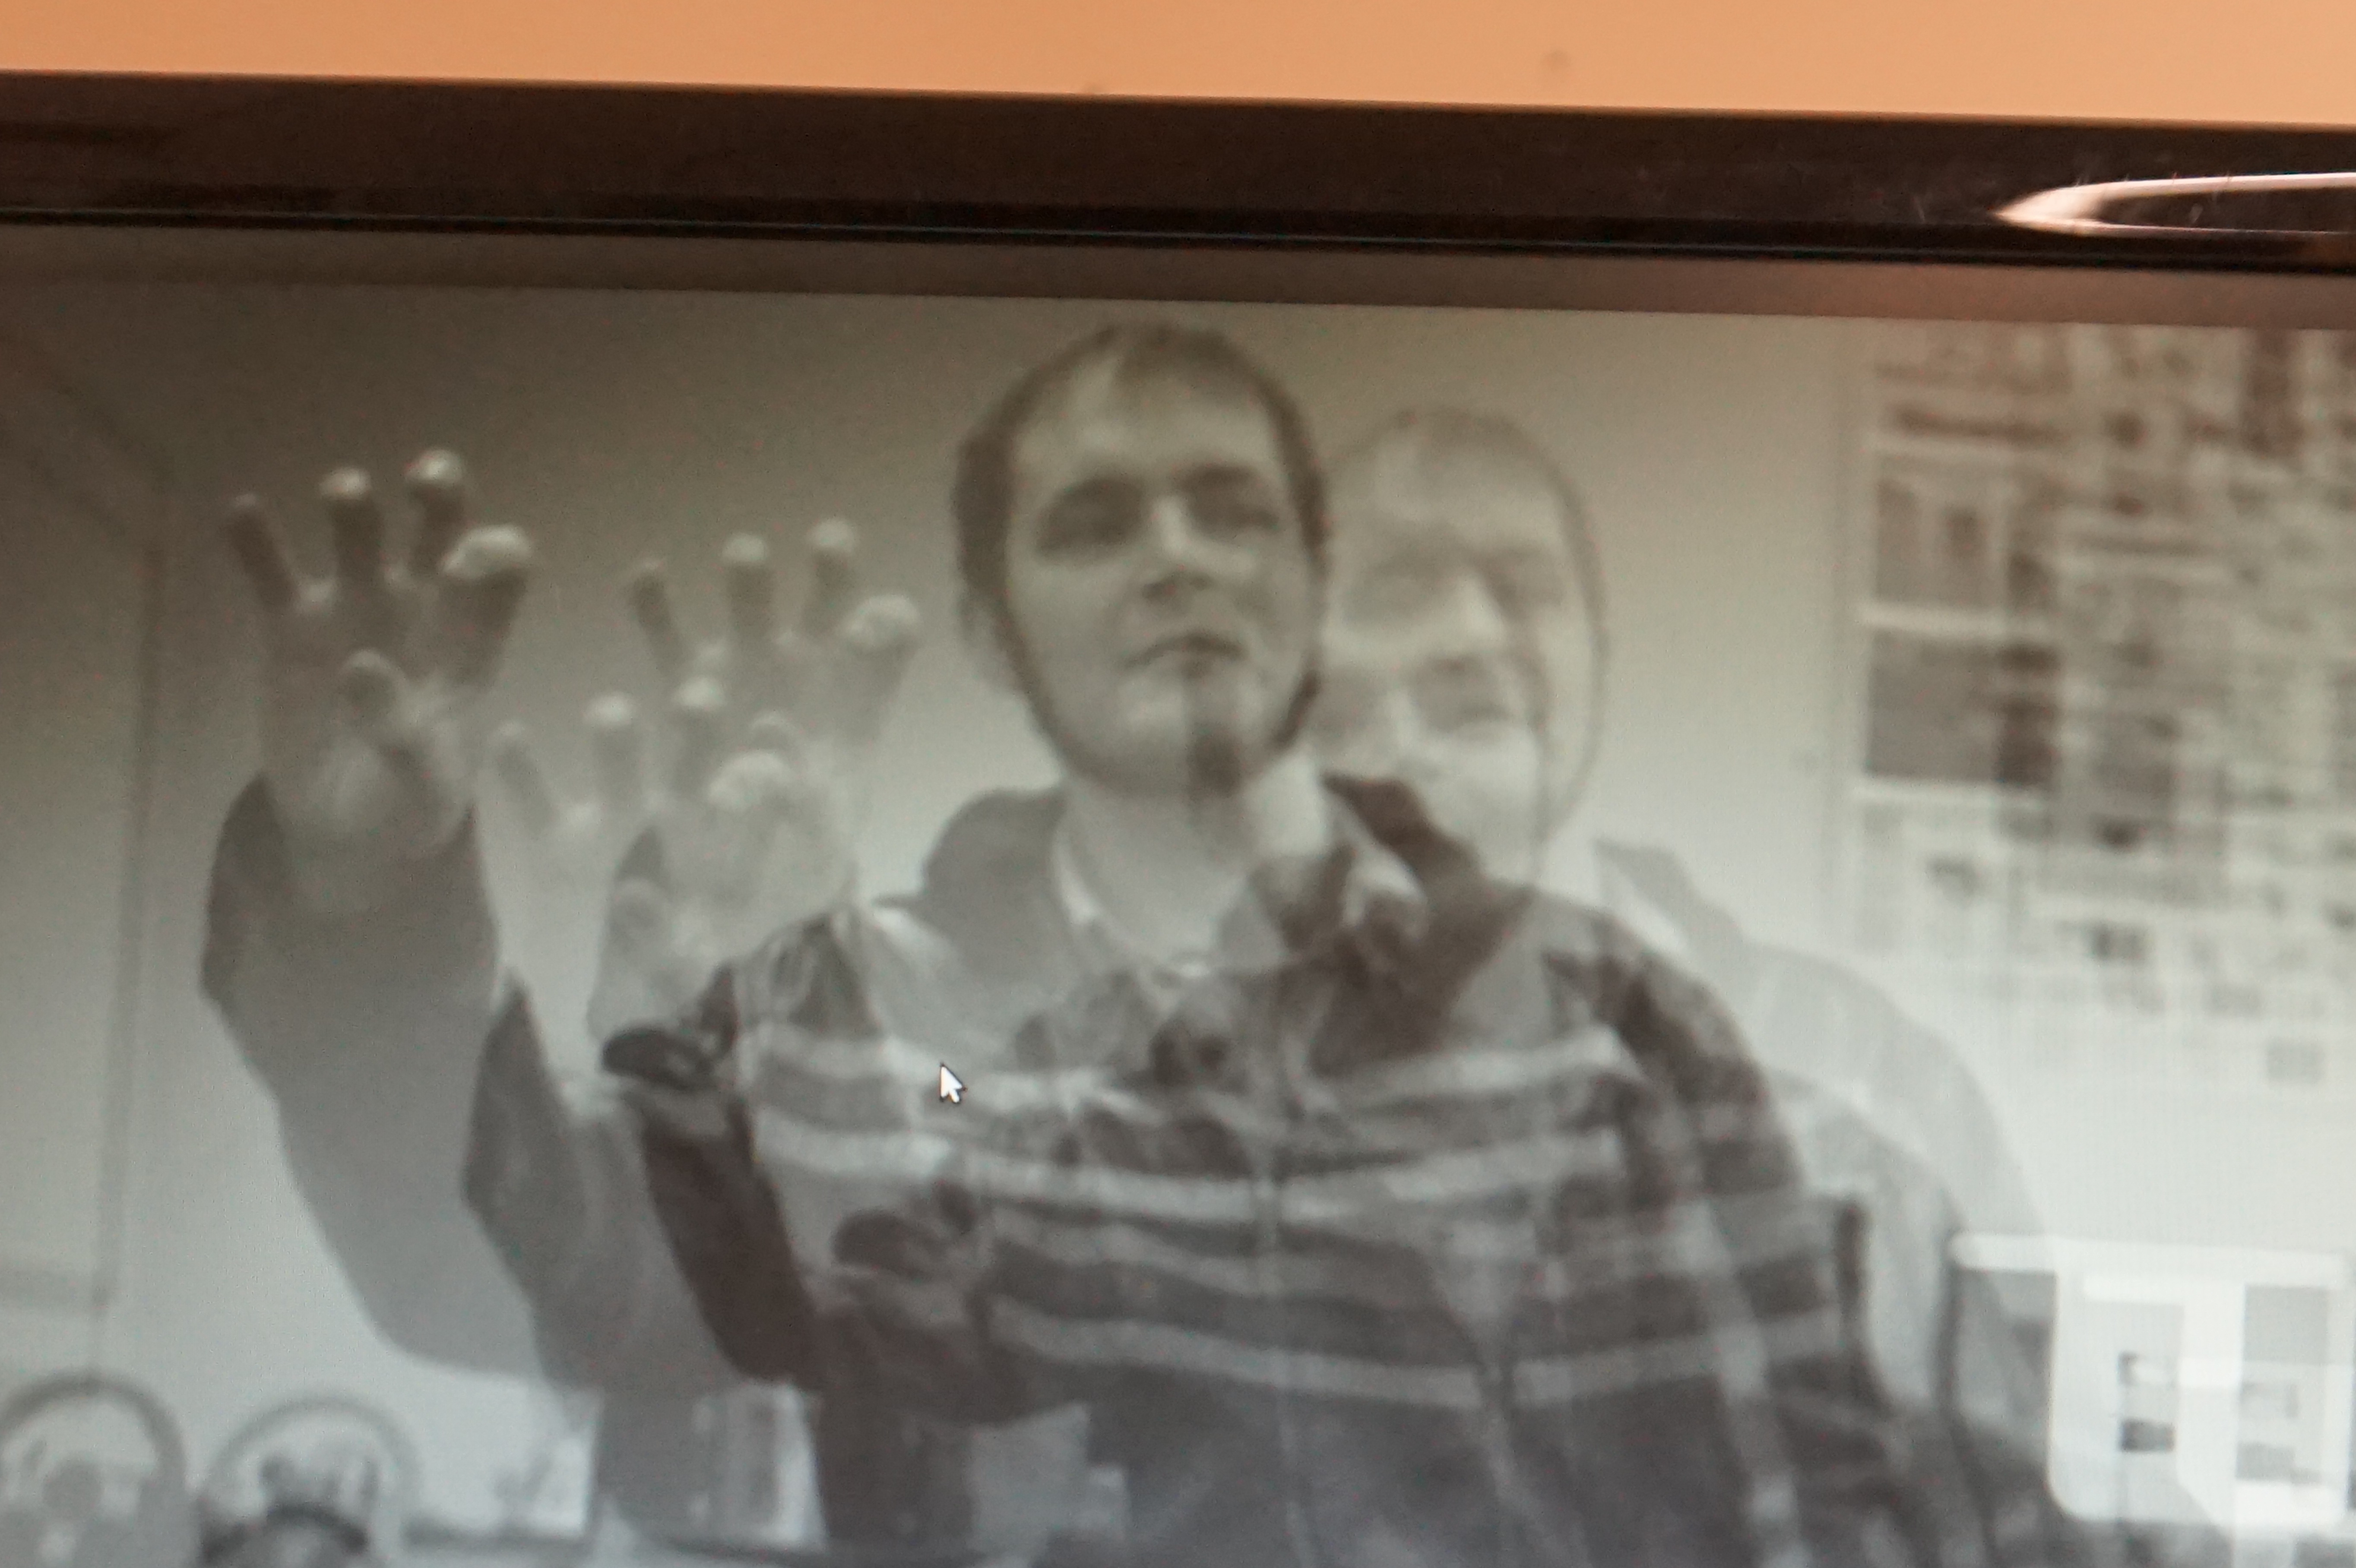
\includegraphics[width=0.6\textwidth]{images/3_normal.png}
				\end{figure}
				
  \subsection{Engineering Expo Demonstration}
  During a meeting with our Sponsors, the idea for our live demonstration at the engineering expo was created. They expressed that they wanted us to present a live feed that displays the use of overlaying multiple images and having to ability to switch to some other camera feature, such as a zoomed in image. The end idea that was agreed upon, was to create a miniature runway with approach LED lights. The runway would be to scale giving a realistic image of a three degree pitch from the location of the aircraft in air, to the front of the runway. This angle simulates the plane roughly be 200 feet off the ground and about 2400 feet from the front edge of the runway. The approach lights will be leading up to the runway, which we will be able to detect using our NIR camera. We ordered a NIR pass filter for the NIR camera that will allow the NIR light to pass, but blocks out any other light. We will then take this image and overlay it with our daylight normal image of the runway. We will also be able to switch to a camera with a zoom lens to magnify the runway number. This feature can also help assist the pilot in locating the correct landing strip. These different functionalities will be able to display the asymmetrical camera system, which is an important part of arial vision systems.\\
  \par
  We are using a 6x1 wood board that is eight feet long to create the runway on. Currently we have the runway itself painted with the threshold, touch down, fixed distance, and center line markings and the identification number.
   
\section{Problems That Impeded Progress}
  \subsection{System and Code Bugs}
	We had a few code bugs in the system that caused strange output or system failure.\\
	\begin{itemize}
		\item System froze during program exit: Our system didn't uninitialize the hardware properly and ended up freezing up the hardware. This wasn't difficult to fix and simply required us to create an exit function.
		\item Camera output is split: Another issue while quitting our application is improper reinitialization of the cameras. This can cause cameras to act strangely upon restart, such as partitioning their image output in half before sending it to the screen. We have dterminined this to be a problem with our hardware and is fixed by simply never rebooting the system during demo.
	\end{itemize}
   
   \subsection{Jetson TX1 Kernel Recompile}
   We found that the Jetson TX1's operating system had to be recompiled in order to grab full 2048x2048 pixel images from the camera. Without the recompiled kernel we were able to grab images at a lower resolution using the FlyCapture API, but we needed to obtain the higher resolution to match our requirement of 1080 pixels at 30 frames per second. We had to recompile the TX1 kernel with a special version of Linux4Tegra, named "Grinch," to get the output from the USB 3.0 PointGrey camera. The original version of the kernel that was supplied with the TX1 had actually disabled support to the USB 3.0 port and was only allowing it to be used as a USB 2.0. The recompile of the kernel proved to be a difficult task, and we still had some connection and display issues with the video stream on the TX1. Despite these setbacks, we were able to get a much better video output on the TX1.
   
   \subsection{Jetson TX1 Manufacturer Error}
   Development on the Jetson TX1 began slowly as we found that our first TX1 had a manufacturing problem, preventing it from connecting to wifi and causing unacceptable system lag. We notified our instructor who gave us another board that also turned out to be defective in the same way. We then had to return the Jetson TX1 we currently had, and order a brand new board. In the meantime we were working with the TK1, until the new fully functional TX1 arrived. When it arrived and had been tested to detect that the manufacturer error wasn't present, we were finally able to switch development from the TK1 to the TX1.
   
   \subsection{Jetson TX1 and PointGrey Camera Compatibility}
   After getting video output using the Jetson TX1's on-board camera, our next step was to interact with the USB 3.0 PointGrey camera. Once we got the PointGrey camera and the TX1 to interface with each other, we ran into the issue of getting the TX1 to register the camera and to display an image from it. We were finally able to get a video output from the PointGrey camera after realizing we were missing two big elements. To fix the issue, we first needed to recompile the Linux kernel to increase the USB buffer size to accommodate for the higher resolution image capturing from the PointGrey camera, as the on-board camera had a much lower resolution. Secondly, we had to acquire the proper camera software needed from PointGrey directly to interface between the proprietary camera API and OpenCV. After all was said and done, we had generated an output video stream from the USB 3.0 camera. 
   
   \subsection{OpenCV Limiting Frame Rate}
   After further development in OpenCV we found that our visual frame rate was not matching the frame rate that was being logged. The logs were saying we were outputting 30 fps, but the video output was obviously less than that showing significant lag. We determined that this lag was due to a bottleneck when frames were being copied from the CPU to the GPU. Fixing this in OpenCV would've taken some serious investigation into OpenCV's code that we did not have the time for. Therefore, we left the capture and processing system in place, and simply replaced the way we were display the images. We have changed development to two different libraries that are able to replace OpenCV. One is called GLUT and uses OpenGL to create a window and display images on the screen. The other is a low level API that allows us to directly manipulate the frames on the GPU. This API is called CUDA, which is NVIDIA's general purpose GPU API. This allowed us to use a feature called Zero Copy, which allows us to write directly into GPU memory from the host application. Zero copy allows us to write the camera images directly to a buffer that is read by the GPU because the GPU and the CPU share memory. We now have eliminated the need for slow copy procedures, resulting in multiple camera inputs stitched together into one output stream with very high frame rate capabilities that are consistent. Performing image format conversions in-place on the GPU will improve performance further. 
   \subsection{Lens Magnification}
   Once we begin working with our runway model demonstration, we were able to see that our two standard camera lenses were blurry for far away object but very good with near objects. Almost so good that you can see someones finger print when held to the camera. No matter the adjustments we made to the lens, we were not able to get a clear image. Our sponsor recommended using spacer to increase the focal length of the camera and lens system, but even once the spacers were applied it made the focal length even worse giving us a very blurry image. This problem has not been resolved yet and is still on going to create a sharper image. We have discussed using that lens on the NIR camera as the LED lights will be at a closer range to the cameras. 

   \subsection{Proper Latency Testing}
   We originally used a simple Linux time function inside a thread in our software in order to determine what the latency of our system was. After discussing this method with our clients we learned that measuring the framerate using software functions commonly causes problems. Our clients suggested that we should use a high speed camera to measure the latency. The high speed camera would record the monitor as well as a LED blinking on and off, allowing us to mesure how many frames it took after the LED was turned off for the displayed image to show that the LED was off. This method is a surefire way to get the correct latency because it's hard for software to ensure the correct measurements of hardware latency. For our high-speed camera, we borrowed a GoPro Hero4 from our professor and then counted the frames in a video editor.
   
\section{Release Results}
   Our project defines specific latency, frame rate, and resolution requirements in order for our system to be a viable option to replace the current FPGA system. Our end-to-end latency requirement specifies that it should take less than 100ms to capture video from the camera, process it, and display the output stream. Additionally, we are required to process a minimum of 30 frames per second at 1080p resolution. Our goal is to perform as much image processing as we can while maintaining these performance metrics.\\
\par
In order to measure the latency of our application, our software contains a detailed, built-in performance logging system. Each component of the software is separated into polymorphic, class-based, HawkEye modules. Each individual module measures execution time including the time it takes to transfer the results to the next module. The overall latency for each frame is determined by the time it takes for all modules to finish executing from input to output, counted as the sum of the longest path. It is important to measure each individual module's latency as well as the overall latency because not all cameras are going to be subjected to the same filtering algorithms. The additional information will enable us to predict the outcome latency based on the set of modules used. In order to measure the frame rate, we simply count the number of frames processed in a second.\\
\par
Our goal is to support independent image processing of three separate inputs. Rockwell Collins has given us some challenges outside of our requirements, which we will try to implement. We have multiple types of cameras with different lenses: two standard RGB cameras and one NIR (Near infrared) camera. The IR camera will be used to identify high intensity point lights, which we will then overlay onto the processed input from one of the RGB cameras. In the industry, this would be used to identify runway lights for landing aircraft. The third camera would provide a more focused look at the target. The first performance benchmark we need to determine is to simply get three simultaneous camera feeds running at the full 30 frame per second.\\

\begin{center}
	\begin{tabular} { | l | c | c | c | }
	\hline
	\multicolumn{ 4 } { | c | } { Frame Rate} \\
	\hline
	 	                                                      & One Camera       & Two Cameras         & Three Cameras \\ \hline
	USB 3.0 with OpenCV                           & 37 FPS average &          		          &  \\ \hline
	USB 2.0 with OpenCV                           & 11 FPS average  & 10 FPS consistent & 6 FPS \\ \hline
	USB 3.0 with CUDA                               & 40 FPS               & 35 FPS                   & 32 FPS \\ \hline
	USB 3.0 with CUDA and multithreaded & 100-110 FPS      & 50-70 FPS              & 45 FPS \\ \hline
	\end{tabular}
\end{center}

\par

\begin{center}
	\begin{tabular} { | l | c | c | c | }
	\hline
	\multicolumn{ 4 } { | c | } {Total Latency} \\
	\hline
	 	      & One Camera & Two Cameras & Three Cameras \\ \hline
	USB 3.0 &	 16-30 ms       &          	       &  \\ \hline
	USB 2.0 & 26-45 ms       & 38-56 ms        & 42-67 ms \\
	\hline
	\end{tabular}
\end{center}

\par
Note: One-camera usb 2.0 results are shown for comparison purposes.\\
\par
After having poor initial results using OpenCV, we decided to completely implement our own vision processing platform that utilizes GPU optimized video processing with the CUDA library. Our new vision platform takes advantage of the shared memory of the CPU and GPU on the Jetson by using a CUDA feature called Zero Copy. This allows us to create buffers that are shared directly between the CPU and GPU, without having to copy the image every time it is used. We integrated this functionality directly into our camera input system by allocating a shared memory buffer and setting up PointGrey's colorspace conversion to output directly into this buffer. Once the image is in GPU memory, we then are able to perform extremely fast operations on it using the GPU. Finally, we map the CUDA buffer to an OpenGL texture, which is then drawn to the screen.\\
\par
Using CUDA for our image processing system allowed us to meet high performance metrics, as we were able to add new filters with virtually no effect on frame rate or latency. Even a seemingly intensive edge detection algorithm causes a reduction of less than 1 frame per second. However, we were still limited on our frame rate by the input module.The 35-40fps we are now acquiring is acceptable for our requirements, but our cameras are capable of much greater frame rates: up to 166fps at 1080p. By inserting timing measurements into each step in the input module, we were able to determine that the main cause of slowdown is the PointGrey colorspace conversion, which can take up to 30ms to complete depending on the camera. This initially limited us to lower frame rates, but by threading the input module we were able to perform multiple conversions at the same time. This enabled us to achieve much higher frame rates, up to 110fps with a single camera. Our latency increased slightly to about 40ms, but this is still within our 100ms acceptable range.\\
\par
Our new CUDA-based system is extremely fast, and enables us to work on more advanced image processing algorithms. Our current software includes multiple combination filters which blend two images together by averaging their color values, as well as a edge detection filter that was provided by NVIDIA in their CUDA sample code. Even with three camera inputs, two combination filters, and an edge detection filter, we still achieve roughly 35 frames per second without even coming close to our latency requirement. The image in figure 10 below displays this frame rate and the high quality of the image achieved in the output video stream from our Jetson TX1 and USB 3.0 PointGrey camera.\\

\begin{figure}[!ht]
  \caption{Video output from the TX1 running at ~35 fps}
	  \centering
		    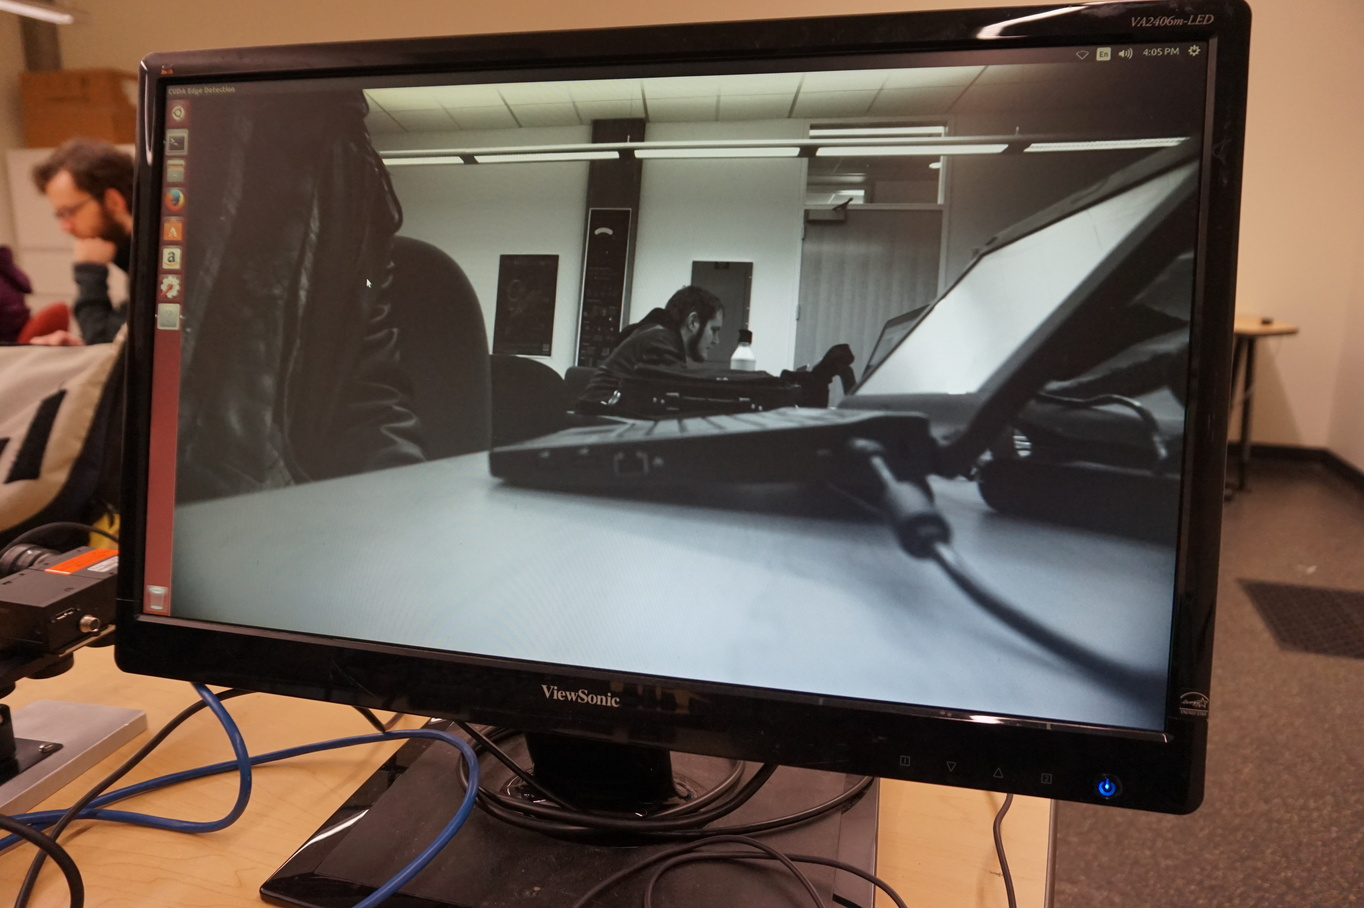
\includegraphics[width=0.6\textwidth]{images/exampleOutputNormalBeta.jpg}
				\end{figure}
  
  \subsection{Implications of Beta Results}
  Now that our frame rate far exceeds our requirement, we can now focus on debugging, increasing stability, and implementing our stretch goals. Our current software works perfectly when it is running, but sometimes it will crash during exit because the GPU cleanup may occur before some of the threads operating on GPU memory have actually terminated. Once we fix these issues, we will then focus on additional improvements. We intend to create a CUDA color space conversion to replace the existing one, which should enable us to maximize our frame rate for all cameras. Then we will focus on our stretch goal of implementing a runway detection filter.

\section{What is left to do}
	
	\subsection{Stretch Goals}
	If time permits, we should have the ability to implement some other functionality that extends our requirements standard. We have developed a plan for some of these, and are considering them as stretch goals. A few of these features have already been implemented or are close to being meet:\\
	\begin{itemize}
		\item Display our video output stream on more than one monitor simultaneously  
		\item Perform an object tracking filter
		\item Design a real-world model to test our cameras on, such as with miniatures (two of our cameras have micro lenses which would be perfect for miniatures)
		\item Display video operation metrics on screen; we currently log these to a file, but it would be easier to demonstrate the capabilities of the SBC if we displayed these on the video stream
		\item Compare the Jetson with different single board computers, which would include re-implementing our code on different platforms and comparing their processing speed and hardware capabilities\\
	\end{itemize}
	
  \subsection{Runway Demonstration}
  For our runway demonstration, we still need to add the approach lights using LED strip lights. These lights will be powered and operated by a Raspberry Pi. We must also create a stable stand to put the cameras on and give them the proper height to match our scale requirements of a 3 degree pitch from the runway. 

  \subsection{Implementing Zoom Lens}
  As part of our runway demo we will have a camera with a zoom lens fixed on the number painted on our runway. The zoom lens will provide a clearer image of the number on the runway for identification. In a real world scenario, the plane may be too far away for the pilot to see the number without a zoom camera, which creates a real world application of zoom lenses. The implementation of a zoom lens in our demo will show that single-board computers can handle practical applications like this.

  \subsection{Fix Image Overlay}
  In another part of our runway demonstration, we will use a zoom lens, an NIR camera, and an RGB camera to produce one output. Because the cameras are spaced far apart relative to the model runway, we will need to implement an overlay function inorder to combine the video produced by the three camera correctly.
	
   \section{Interesting Piece of Code}
   The core of our program is the modular video processing pipeline. This polymorphic object-oriented system allows us to easily implement new video processing algorithms, support for different types of input devices, and new methods of outputting results. It is also responsible for measuring performance of each individual component.\\
   
   \subsection{CUDA based modules}
In our base program, each module is defined in its own class, which is a child class of HawkEye\_Module. Each module has two required parts, the constructor and the run() command, as well as an existing setup() command which can be overloaded as needed. The HawkEye\_CUDA\_Module retains these functions, but provides a default run() method which calls an appropriate runKernel() CUDA function based on the number of inputs and outputs. This is the default functionality for CUDA modules, but the run() function can be overloaded to provide different functionality if desired. \\
   \begin{lstlisting}
   	class MyModule: public HawkEye_CUDA_Module{
	public:
		MyModule(){
			numinputs = 2;
			numoutputs=1;
			setup();
		}  
   \end{lstlisting}
 \par
   The initializer MUST set the number of inputs and outputs. This is extremely important because the setup() function creates the appropriate buffers and sets some internal variables needed by the module class to determine when the needed inputs have been satisfied (and thus when to execute).\\
   \begin{lstlisting}
	   
	// CUDA kernel executed on the GPU
   	__global__ void runKernel(Pixel *output, Pixel *inputa, Pixel *inputb){
	    index = blockIdx.x*blockDim.x + threadIdx.x;
		output[index]=inputa[index]/2 + inputb[index]/2;
	}
	
   \end{lstlisting}
 \par
   This code describes a GPU accelerated module that would take two images and combine them together by a simple averaging method. The HawkEye\_CUDA\_Module class automatically allocates output buffers in shared CPU/GPU memory based on the number of inputs and outputs defined in the class constructor. This particular code sample is what is known as a CUDA kernel, which means that it is compiled by the NVIDIA compiler and executed on the GPU. The \_\_global\_\_ specifier tells the compiler that it is a CUDA section. The runKernel function is an overloaded virtual function that the HawkEye\_CUDA\_Module class sets up and runs in a manner completely transparent to the algorithm implementer. The only thing the implementer needs to know about are the blockIdx,blockDim, and threadIdx variables, which are part of the CUDA system. These variables define the different GPU threads' operating locations in the buffer.\\
 \par
	Our system does not limit users to our built in CUDA kernel execution model. The user can choose to implement a more complex algorithm that includes a mixture of CUDA and CPU based operations. Also, we maintain compatibility with our OpenCV module system by automatically creating a OpenCV Mat object around our shared memory buffers. This allows the user to take advantage of OpenCV's built in filters and matrix operations, although we do not actually use them in our modules due to performance issues. \\

   \subsection{JSON configuration}
Once such a module is defined, it can then be added to the parser. Currently this is a hardcoded list of module names which checks an input type name string against the predefined types and creates the associated module, however we have plans to implement a dynamically-loaded module system that allows adding new modules automatically via a dynamically linked library. After the module is added to the parser, instances can then be created in the JSON configuration file. In order to create an instance, an entry is added to the ''modules'' section of the config file.\\   
\par
A JSON configuration for our program consists of three sections: The ''modules'' section, which defines named instances of HawkEye\_Modules, the ''start'' section, which tells the program to start a camera or input, and the connections section, which defines where the output(s) from each module goes to (as a module could have multiple outputs, and some modules require multiple inputs).\\
   \begin{lstlisting}
   	{
		''modules'':{
			''MyModule_instance'':''MyModule'',
			''inputModule'':''camera'',
			''outputModule'':''basicOutput''
		},
		''start'':''inputModule'',
		''inputModule'':{
			''output0'':''MyModule_instance0''
		},
		''MyModule_instance'':{
			''output0'':''outputModule0''
		}
	}
   \end{lstlisting}
 \par 
   In this example, we define two camera inputs, a combination algorithm module (as defined above in the previous code example), and an output window module. The start section tells the program that it needs to run both camera inputs, which it does separately. The code immediately after the start section tells the program to connect output 0 of inputModule1 to input 0 of MyModule\_instance, output 0 of inputModule2 to input 1 of MyModule\_instance, and the output of MyModule\_instance to the display module. When the program is executed, it will capture input from both cameras, combine it using MyModule, and then display it to a window. This configuration system makes it easy to implement complex networks of algorithm modules, and makes it so that any reconfiguration of the modules does not require a recompile of the software. This also defines the names used by the logger, in this case inputModule1, inputModule2, MyModule\_instance, and outputModule. These names can be anything the user decides to define, as long as they are different.
				
   \end{document}

